%%%% ijcai26.tex
\typeout{IJCAI--ECAI 26 Instructions for Authors}

% These are the instructions for authors for IJCAI--ECAI 26.

\documentclass{article}
\pdfpagewidth=8.5in
\pdfpageheight=11in

% The file ijcai26.sty is a copy from ijcai22.sty
% The file ijcai22.sty is NOT the same as previous years'
\usepackage{ijcai26}
\usepackage[table]{xcolor}
% Use the postscript times font!
\usepackage{times}
\usepackage{soul}
\usepackage{url}
\usepackage[hidelinks]{hyperref}
\usepackage[utf8]{inputenc}
\usepackage[small]{caption}
\usepackage{graphicx}
\usepackage{amsmath}
\usepackage{amsthm}
\usepackage{booktabs}
\usepackage[switch]{lineno}
% \usepackage{colortbl}
\usepackage{algorithm}
\usepackage{algorithmic}
\usepackage{amssymb}
\newcommand{\cmark}{$\checkmark$}
\newcommand{\xmark}{$\times$}
\usepackage{enumitem}            % 精细控制列表间距(您使用了\itemsep)
\usepackage{subcaption}          % 子图支持(如果有多图)
\usepackage{xcolor}              % 颜色支持(某些模板需要)
\usepackage{stmaryrd}           % 语义符号(可选)
\usepackage{float}              % 浮动体控制
 \usepackage[table]{xcolor}
 \usepackage{booktabs}
 \usepackage{colortbl}
 \usepackage{multirow}
 \usepackage{pifont}

% light helpers
 \newcommand{\best}[1]{\cellcolor{green!12}\textbf{#1}}
 \newcommand{\good}[1]{\cellcolor{gray!10}#1}
 \newcommand{\bad}[1]{\cellcolor{red!10}#1}
 \newcommand{\up}{\textcolor{green!50!black}{\ding{115}}}
 \newcommand{\down}{\textcolor{red!70!black}{\ding{55}}}
\newcommand{\ci}[2]{$#1 \pm #2$}   % 显示为 0.1x ± 0.0x
% 定义方法标签显示
\newcommand{\method}[1]{\texttt{#1}}

% Comment out this line in the camera-ready submission
\linenumbers

\urlstyle{same}

% the following package is optional:
%\usepackage{latexsym}

% See https://www.overleaf.com/learn/latex/theorems_and_proofs
% for a nice explanation of how to define new theorems, but keep
% in mind that the amsthm package is already included in this
% template and that you must *not* alter the styling.
\newtheorem{example}{Example}
\newtheorem{theorem}{Theorem}

% Following comment is from ijcai97-submit.tex:
% The preparation of these files was supported by Schlumberger Palo Alto
% Research, AT\&T Bell Laboratories, and Morgan Kaufmann Publishers.
% Shirley Jowell, of Morgan Kaufmann Publishers, and Peter F.
% Patel-Schneider, of AT\&T Bell Laboratories collaborated on their
% preparation.

% These instructions can be modified and used in other conferences as long
% as credit to the authors and supporting agencies is retained, this notice
% is not changed, and further modification or reuse is not restricted.
% Neither Shirley Jowell nor Peter F. Patel-Schneider can be listed as
% contacts for providing assistance without their prior permission.

% To use for other conferences, change references to files and the
% conference appropriate and use other authors, contacts, publishers, and
% organizations.
% Also change the deadline and address for returning papers and the length and
% page charge instructions.
% Put where the files are available in the appropriate places.


% PDF Info Is REQUIRED.

% Please leave this \pdfinfo block untouched both for the submission and
% Camera Ready Copy. Do not include Title and Author information in the pdfinfo section
\pdfinfo{
/TemplateVersion (IJCAI.2026.0)
}

\title{ScholarArena: Evidence-Gated, Replayable Multi-Party Scientific Discourse}

% Single author syntax
\author{
    Author Name
    \affiliations
    Affiliation
    \emails
    email@example.com
}

% Multiple author syntax (remove the single-author syntax above and the \iffalse ... \fi here)
\iffalse
\author{
First Author$^1$
\and
Second Author$^2$\and
Third Author$^{2,3}$\And
Fourth Author$^4$\\
\affiliations
$^1$First Affiliation\\
$^2$Second Affiliation\\
$^3$Third Affiliation\\
$^4$Fourth Affiliation\\
\emails
\{first, second\}@example.com,
third@other.example.com,
fourth@example.com
}
\fi

\begin{document}

\maketitle

\begin{abstract}
	Large language models are increasingly deployed to assist peer review, rebuttal, and meta-review, but most systems still operate in free-form text. As a result, citations are often treated as optional annotations rather than enforceable contracts, cross-round context drifts in ways that cannot be deterministically replayed, and tool failures frequently lead to fail-open behavior. These weaknesses are amplified in scientific discourse, where unsupported factual statements degrade accountability and integrity risks such as prompt injections embedded in papers can steer interactions.
	%
	We present \textsc{ScholarArena}, a framework for evidence-gated and replayable multi-party scientific discussion. \textsc{ScholarArena} treats evidence production as executable. An Offline Foundry inverts raw multi-round dialogues into issue-threaded semantic instances, mines evidence needs, compiles a deterministic library of Primitives and Skills via sandboxed candidate--test gating, and re-grounds supervision by executing the library to produce citable Observations with locatable provenance. An Online Arena deploys a role-conditioned policy that plans intents and skill calls and emits structured actions whose factual fields are hard-gated, so every claim must cite an Observation or the policy can only produce auditable next steps. Per-thread ledgers and finite-state control enable deterministic replay and fine-grained attribution, while meta coordination is restricted to ledger state to limit cross-agent instruction channels.
	%
	Experiments in an ICLR-style three-role setting show that \textsc{ScholarArena} improves evidence precision and decision consistency, reduces unsupported claims, and increases robustness to injection-oriented perturbations against strong baselines. Code is available at \url{anonymous.4open.science/r/Repository-7BFB}.
\end{abstract}


\section{Introduction}

\begin{figure}[t]
	\centering
	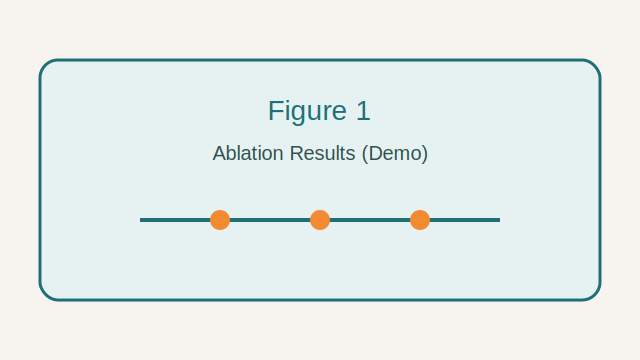
\includegraphics[width=1\columnwidth]{fig1.pdf}  % 调整路径和宽度
	\caption{Illustrative examples of multi-agent peer review: free-form assistants may fail open (hallucinated ablations, uncited novelty claims, injection-steered meta), while ScholarArena enforces a hard evidence gate, producing either evidence-backed statements or auditable next-step plans.}
	\label{fig:teaser}
\end{figure}

Scientific progress is mediated by structured yet highly interactive discourse: reviewers request clarifications and evidence, authors respond with revisions and rebuttals, and meta-reviewers coordinate threads toward a final decision. As the scale and pace of submissions continue to increase, large language models (LLMs) are now routinely used to assist this process (e.g., summarizing papers, drafting responses, or triaging issues). However, the dominant interaction modality remains \emph{free-form}: models produce fluent text that may mix grounded facts with plausible-sounding but unsupported statements, and multi-round dialogue often relies on implicit references and drifting context. In peer-review settings, these failures are especially costly—misattributed claims can distort scientific conclusions, and untraceable model behavior undermines accountability.

A first line of work addresses faithfulness via retrieval-augmented generation and citation-backed answers, aiming to make outputs auditable by attaching supporting passages (e.g., ALCE) \cite{gao-etal-2023-enabling}. Yet recent evidence suggests that \emph{producing citations is not equivalent to being grounded}: automatic attribution evaluation remains difficult \cite{li-etal-2024-attributionbench}, and large-scale audits show substantial rates of unsupported statements even when models cite sources \cite{wu2025sourcecheckup}. Meanwhile, long-context settings amplify the need for fine-grained, sentence/span-level provenance; recent systems improve citation granularity and quality, but still largely treat evidence as passive text rather than an enforceable contract \cite{zhang2025longcite,chuang-etal-2025-selfcite}. Complementary “traceability” frameworks further motivate claim-level grounding as a practical interface for verification \cite{chu-etal-2026-etracer}.

A second line of work studies tool-augmented agents and multi-agent collaboration \cite{yao2023react,wu2023autogen,chen2024agentverse}, and execution-based evaluation for validating tool use \cite{jimenez2024swebench,yang2024sweagent}. However, many agentic systems still rely on unconstrained cross-round prompting and unstructured memory, making it difficult to (i) deterministically replay what happened, (ii) localize which evidence supported which claim, and (iii) enforce “fail-closed” behavior when evidence is missing or tool execution fails. In scientific discussion, these limitations intersect with emerging integrity and security concerns: recent studies demonstrate that LLM-assisted reviewing pipelines can be manipulated by hidden prompt injections embedded in papers, yielding biased or steered reviews \cite{collu-etal-2025-publishtoperish,keuper-2025-promptreview}.

In this paper, we propose \textbf{ScholarArena}, a framework for \emph{verifiable} multi-party scientific discussion that treats evidence production as \emph{executable} and enforces a \emph{hard evidence gate} over all factual fields. ScholarArena makes two deliberate design choices. First, it targets assistance for \emph{multiple participants} (Reviewer/Author/Meta) throughout issue-threaded discussion rather than generating a monolithic “review.” Second, it explicitly models missing evidence and execution failures as first-class outcomes, forcing the policy to respond with only auditable next steps when grounding is unavailable.

Concretely, ScholarArena structures interaction around (1) an \emph{Offline Foundry} that compiles deterministic capabilities and re-writes supervision with executable provenance, and (2) an \emph{Online Arena} that executes issue threads under ledger-based state control. The key mechanism is \emph{evidence gating}: instead of merely attaching citations post hoc, ScholarArena restricts the action space so that any factual claim must be justified by an Observation localized to $\mathcal{C}$. This “fail-closed” contract is conceptually aligned with recent calls for verifiable interfaces (e.g., claim-level grounding and proof-carrying outputs) \cite{chu-etal-2026-etracer,solatorio-2025-pcn}, but is operationalized here as an end-to-end training and deployment framework for peer-review-style discourse.

Our main contributions are:
\begin{itemize}[leftmargin=*,itemsep=0.2em]
	\item \textbf{We introduce an evidence-gated interaction model for multi-party scientific discussion.}
	ScholarArena represents every step as an executable Move that separates intent selection, deterministic tool execution, and evidence-conditioned action emission, and it enforces a fail-closed constraint in which factual fields are admissible only when supported by citable Observations.
	
	\item \textbf{We formalize replayable issue-thread execution with explicit provenance and controllable state.}
	We design a per-issue ledger and a finite-state controller that externalize cross-round context into structured state, enabling deterministic replay, localized evidence attribution, and principled handling of missing evidence and execution failures.
	
	\item \textbf{We propose an Offline Foundry that compiles deterministic capabilities and rewrites supervision with executable provenance.}
	Starting from inverted dialogue instances, the Foundry mines evidence needs, compiles Primitives and Skills through candidate--test gating, and re-grounds each instance by executing the compiled library to replace approximate evidence pointers with locatable provenance.
	
	\item \textbf{We provide an integrity-aware coordination mechanism that limits cross-agent instruction channels.}
	The Meta role schedules threads using only ledger states and thread identifiers, reducing cross-round drift and constraining prompt-injection-style contamination pathways \cite{collu-etal-2025-publishtoperish,keuper-2025-promptreview}.
\end{itemize}

\section{Related Work}
\label{sec:related}

\paragraph{Evidence-grounded generation and fine-grained attribution.}
A large body of work aims to improve the faithfulness and auditability of LLM outputs by coupling generation with explicit evidence and citations.
ALCE formalizes end-to-end systems that retrieve supporting passages and produce cited answers, together with automatic metrics for citation quality \cite{gao-etal-2023-enabling}.
However, AttributionBench shows automatic attribution evaluation remains challenging even for strong LLMs \cite{li-etal-2024-attributionbench}, and SourceCheckup-like pipelines further highlight substantial rates of unsupported statements despite citation outputs \cite{wu2025sourcecheckup}.
Recent efforts also push toward more fine-grained, sentence/span-level citations in long-context QA \cite{zhang2025longcite}, and post-hoc revision frameworks such as RARR improve attribution by iteratively researching and revising model claims \cite{gao-etal-2023-rarr}.
Self-reflective retrieval approaches (e.g., Self-RAG) additionally integrate retrieval decisions and critique signals during generation \cite{asai2024selfrag}.
In contrast, ScholarArena treats evidence production as \emph{executable} and applies a \emph{hard evidence gate} to the produced actions.
Concretely, any factual field in an action must be supported by a citable Observation; otherwise, the policy is constrained to produce only auditable follow-ups such as clarification requests, evidence plans, or conditional commitments.

\paragraph{Tool-augmented agents and executable verification.}
Tool-using and multi-agent systems have been widely explored for complex task decomposition and collaborative behaviors \cite{yao2023react,wu2023autogen,chen2024agentverse}.
These lines of work highlight the effectiveness of combining LLM policies with external tools and role-based interaction, but many systems still rely on free-form cross-round instructions and unstructured memory, which can blur provenance and hinder deterministic replay.
In parallel, test-driven and execution-based evaluation has become a practical mechanism for validating tool-augmented behavior in realistic settings \cite{jimenez2024swebench,yang2024sweagent}.
ScholarArena instead adopts a minimal, auditable interface: interactions are mediated by a per-issue ledger and a finite-state controller, while capabilities are compiled into deterministic Primitives/Skills with replayable execution and locatable provenance.
This design prioritizes verifiability through executable traces and explicit evidence localization, rather than relying on unconstrained dialogue history.


\paragraph{LLMs for peer review and scientific discussion, and safety considerations.}
Recent systems and datasets have started to operationalize LLMs for peer-review-like tasks, ranging from specialized review generators (e.g., OpenReviewer) \cite{idahl2024openreviewer} to review-driven conversation synthesis for multi-turn training \cite{wu-etal-2025-review}, and full-stage peer review/rebuttal corpora that capture reviewer--author interactions \cite{zhang2025re2}.
In parallel, multiple works highlight integrity risks of LLM-assisted reviewing, including prompt-injection-style manipulation and broader vulnerabilities in automated review pipelines \cite{ye2024are,gibney2025scientists}.
Relative to OpenReviewer, Review-Instruct, and Re$^2$, ScholarArena does not aim to generate complete reviews.
Instead, it supports multi-party scientific discussion by structuring interactions into issue threads with ledger-based state, role-conditioned moves, and evidence-gated, citation-backed actions.


\section{ScholarArena}
\label{sec:method}

% =========================
% Fig. (System loop overview) placeholder: place near the beginning of Method.
% =========================

\begin{figure*}[t]
	\centering
	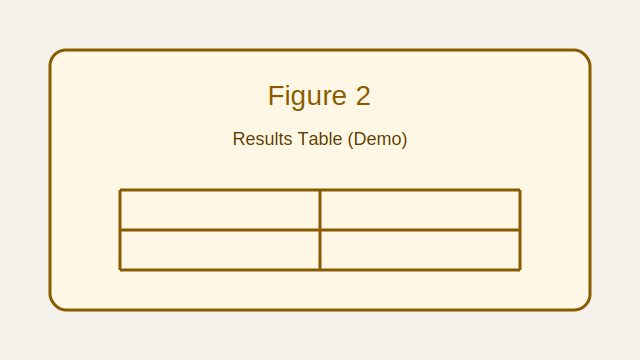
\includegraphics[width=0.95\textwidth]{fig2.pdf}
	\caption{ScholarArena compiles a tested library $\mathcal{L}^{(\star)}$ and executable Observations in an Offline Foundry to re-ground instances into $\mathcal{A}^{(\star)}$, then runs issue-threaded discussion in an Online Arena with ledger+FSM and field-level hard evidence gating, producing replayable trajectory logs and feeding failures back to compilation.}
	\label{fig:overview}
\end{figure*}

ScholarArena targets \emph{verifiable} fact-checking and \emph{executable} action orchestration in scientific discussions, with two deliberate scoping choices: (1) unlike prior multi-agent systems~\cite{chen2024agentverse}, it is designed to assist \emph{multiple participants} throughout the scientific discussion process, and (2) it does not aim to replace participants or automate human judgment on subjective dimensions such as novelty, significance, or importance. Rather than treating missing evidence or failed execution as an exception, the framework explicitly models such outcomes and forces the interaction policy to return only auditable follow-ups (e.g., clarification requests or conditional commitments) under hard evidence constraints. 

Next, we will introduce our proposed behavior inversion for replayable semantic instances, the offline foundry for capability compilation and evidence re-grounding, evidence-gated role-conditional training objectives, and the online arena for ledger-based multi-agent thread execution. The overall framework is shown in Figure~\ref{fig:overview}.
\subsection{Problem Setting and Behavior Inversion}
\label{sec:inversion}

\paragraph{Paper context.}
Given a paper, we parse it into a structured context
$\mathcal{C}=\{c_j\}_{j=1}^{|\mathcal{C}|}$, where each segment $c_j$ is a typed unit (e.g., paragraph, table, figure, caption, reference) with a stable identifier and locatable span for provenance.

\paragraph{Raw dialogue log as the initial input.}
Let the complete peer-review dialogue log be
$\mathcal{D}^{raw}=\{(r_t, u_t)\}_{t=1}^{T}$,
where $r_t\in\{\textsc{Reviewer},\textsc{Author},\textsc{Meta}\}$ and $u_t$ is the utterance at turn $t$.
ScholarArena does \emph{not} assume $\mathcal{D}^{raw}$ is directly usable for supervised learning due to implicit references, drifting wording, and non-replayable free-text memory.

\paragraph{Semantic behavior instances (via Inversion).}
We apply an inversion model $\mathcal{I}$ to convert $\mathcal{D}^{raw}$ into replayable semantic behavior instances,
\begin{equation}
	\mathcal{A}^{(0)}=\mathcal{I}(\mathcal{D}^{raw},\mathcal{C}),\quad
	a=\big(r,i,\text{intent},x,\rho^{(0)},\kappa\big),
	\label{eq:behavior}
\end{equation}
where $r$ is the role, $i$ is the issue-thread identifier, $\text{intent}\in\mathcal{I}\!nt$ is a discrete policy label (e.g., \textsf{RequestEvidence}), $x$ is the localized linguistic behavior (a canonicalized short span derived from $u_t$), and $\kappa\in\{1,\dots,T\}$ preserves the total order inherited from $\mathcal{D}^{raw}$ for deterministic replay.
$\rho^{(0)}$ is an approximate evidence pointer (possibly empty), which will be rewritten by executable provenance in the Offline Foundry (Sec.~\ref{sec:foundry}).
This factorization ensures \emph{replayability}: thread evolution depends only on $(a,\mathcal{C})$ and the ledger state (Sec.~\ref{sec:arena}), rather than unstable free-text context.


\subsection{Offline Foundry}
\label{sec:foundry}

The Offline Foundry builds a capability library for evidence production and converts the inverted instances into an evidence-grounded supervision set $\mathcal{A}^{(\star)}$ by rewriting $\rho$ with executable provenance. This stage precedes supervised fine-tuning and is re-invoked after Online Arena runs to incorporate newly surfaced evidence needs (Fig.~\ref{fig:overview}).

\paragraph{Observation representation.}
All system-citable evidence is represented as an Observation
\begin{equation}
	o=\big(\text{type},\text{payload},\text{prov},\text{status}\big),
	\label{eq:observation}
\end{equation}
\noindent where $\text{prov}\subseteq\{1,\dots,|\mathcal{C}|\}$ is a set of segment identifiers in $\mathcal{C}$ that localizes the supporting evidence, and $\text{status}\in\{\texttt{ok},\texttt{missing},\texttt{fail}\}$ indicates the executor outcome: \texttt{ok} means the evidence is successfully located; \texttt{missing} means no matching evidence can be located in $\mathcal{C}$ under the issued query (often because the dialogue requests information beyond the paper, e.g., newly added experiments not present in the current version); \texttt{fail} indicates deterministic execution failure (e.g., parsing/runtime errors).

\paragraph{Capability library.}
We maintain a two-layer library $\mathcal{L}=(\mathcal{P},\mathcal{S})$.
A \emph{Primitive} $p\in\mathcal{P}$ is a deterministic operator $p(\mathcal{C},\phi)\rightarrow o$ (e.g., span retrieval, table extraction, keyword retrieval).
A \emph{Skill} $s\in\mathcal{S}$ is an intent-oriented deterministic orchestration
\begin{equation}
	s(\mathcal{C},\phi)\Rightarrow \mathrm{DAG}(\mathcal{P},\mathcal{C}\!trl)\rightarrow o,
	\label{eq:skill_dag}
\end{equation}
where a directed acyclic graph (DAG) specifies an execution order that composes multiple primitives and controlled subroutines.
$\mathcal{C}\!trl$ denotes controlled LLM subroutines used only to expand, aggregate, or normalize the \emph{observed} evidence into the fields of $o$; they cannot introduce standalone claims that bypass observation. The temperature for these subroutines is set to 0.

\paragraph{Mining evidence needs.}
For each instance $a=(r,i,\text{intent},x,\rho^{(0)},\kappa)$, we derive an evidence need through a deterministic mapper
\begin{equation}
	u=\Psi(\text{intent},x,\rho^{(0)}),\quad u\in\mathcal{U},
	\label{eq:need}
\end{equation}
where $\Psi$ specifies what must be observed to support or refute the behavior (e.g., locating the exact definition of a metric).

\paragraph{Executable artifact compilation.}
Given a need $u$, a compiler proposes candidate artifacts $\{spec,code,tests\}$ for either a Primitive or a Skill, and we accept a candidate only if it passes sandboxed tests
\begin{equation}
	\begin{aligned}
		\{spec,code,tests\} &\leftarrow \mathcal{L}_{comp}(u),\\
		\textsc{SandboxRun}(code,tests) &\in \{\texttt{pass},\texttt{fail}\}.
	\end{aligned}
	\label{eq:eac}
\end{equation}
This test-based acceptance is consistent with execution-based evaluation and verification setups where candidate solutions are validated by running suites in a sandboxed environment~\cite{jimenez2024swebench}. If a candidate fails, the sandbox trace is used as structured feedback for iterative repair.

\paragraph{Evidence re-grounding.}
After updating the library to $\mathcal{L}^{(\star)}$, we re-ground each behavior instance by executing a skill call derived from $(\text{intent},x)$,
\begin{equation}
	\text{call}(a)=\Gamma(\text{intent},x),\quad
	o\leftarrow \textsc{Exec}(\text{call}(a),\mathcal{C};\mathcal{L}^{(\star)}),
	\label{eq:reground_exec}
\end{equation}
and rewrite the evidence pointer as
\begin{align}
		\rho^{(\star)}=\begin{cases}
			\text{prov}(o), & o.\text{status}=\texttt{ok},\\
			\emptyset, & \text{otherwise},
		\end{cases}\\
		a^{(\star)}=\big(r,i,\text{intent},x,\rho^{(\star)},\kappa\big).
		\label{eq:rho_rewrite}
\end{align}

The resulting set $\mathcal{A}^{(\star)}=\{a^{(\star)}\}$ is grounded in executable provenance, since any non-empty $\rho^{(\star)}$ is backed by an Observation whose provenance is locatable in $\mathcal{C}$.

% =========================
% Algorithm (Offline Foundry) - compact.
% =========================
\begin{algorithm}[t]
	\caption{Offline Foundry loop}
	\label{alg:foundry}
	\begin{algorithmic}[1]
		\REQUIRE Context $\mathcal{C}$; instances $\mathcal{A}^{(0)}$; library $\mathcal{L}=(\mathcal{P},\mathcal{S})$; compiler $\mathcal{L}_{comp}$
		\ENSURE Updated library $\mathcal{L}^{(\star)}$; grounded instances $\mathcal{A}^{(\star)}$
		\STATE Mine needs: $\mathcal{F}\leftarrow \{\Psi(\text{intent},x,\rho^{(0)}) : a\in \mathcal{A}^{(0)}\}$
		\FOR{each $u\in\mathcal{F}$}
		\STATE $\{spec,code,tests\}\leftarrow \mathcal{L}_{comp}(u)$
		\IF{$\textsc{SandboxRun}(code,tests)=\texttt{pass}$}
		\STATE Add candidate to $\mathcal{P}$ or $\mathcal{S}$
		\ELSE
		\STATE Repair using sandbox traces
		\ENDIF
		\ENDFOR
		\STATE $\mathcal{L}^{(\star)}\leftarrow (\mathcal{P},\mathcal{S})$
		\FOR{each $a\in\mathcal{A}^{(0)}$}
		\STATE $o\leftarrow \textsc{Exec}(\Gamma(\text{intent},x),\mathcal{C};\mathcal{L}^{(\star)})$
		\STATE Rewrite $\rho$ by Eq.~\eqref{eq:rho_rewrite} to obtain $a^{(\star)}$
		\ENDFOR
		\STATE $\mathcal{A}^{(\star)}\leftarrow \{a^{(\star)}\}$
	\end{algorithmic}
\end{algorithm}


\subsection{Policy Training with Evidence-Gated Supervision}
\label{sec:training}

We train a single role-conditioned policy $\pi_\theta$, where the role identifier $r$ selects the behavioral mode (\textsc{Reviewer}/\textsc{Author}/\textsc{Meta}). Training pairs are obtained by deterministically replaying issue-thread trajectories reconstructed from $\mathcal{A}^{(\star)}$.

\paragraph{Thread ledger and finite-state control.}
For each issue $i$, we maintain a minimal ledger state together with a finite-state machine (FSM) that encodes the coarse interaction phase:
\begin{align}
	S_i^t &= \big(\text{tag}_i,\ \mathcal{L}_i^t,\ \eta_i^t,\ \text{phase}_i^t\big), \nonumber\\
	\mathcal{L}_i^t &= \big(\mathcal{O}_i^t,\mathcal{R}_i^t,\mathcal{K}_i^t,\text{sev}_i^t\big).
	\label{eq:state}
\end{align}
$\mathcal{O}$ is the set of citable Observations, $\mathcal{R}$ is the active request set, $\mathcal{K}$ is the commitment set, $\text{sev}$ is a discrete severity label, and $\eta_i^t$ is a remaining interaction quota.
The phase takes values in the four-state FSM
\begin{equation}
	\begin{aligned}
		\text{phase}_i^t \in \{&\texttt{Open},\ \texttt{EvidencePending},\\
		&\texttt{Negotiation},\ \texttt{Closed}\},
	\end{aligned}
	\label{eq:fsm}
\end{equation}
and is updated by a deterministic transition function $S_i^{t+1}=\mathcal{T}(S_i^t,o_t,y_t)$.

\paragraph{Intent--skill planning and evidence-conditioned action.}
Each interaction step (Move) is factorized into planning, execution, and action:
\begin{equation}
	\text{Move}_t=\big(\text{intent}_t,\ \text{skill\_call}_t,\ o_t,\ y_t\big).
	\label{eq:move}
\end{equation}

Compared with free-form \emph{thought--action} traces (e.g., ReAct-style prompting \cite{yao2023react}), our policy exposes only the minimal \emph{auditable} interface: it first selects a structured intent and an executable skill call, then conditions the subsequent action on the returned Observation.
Formally,
\begin{equation}
	\begin{aligned}
		(\text{intent}_t,\text{skill\_call}_t) &\sim \pi_\theta(\cdot \mid r,S_i^t,\mathcal{C}),\\
		o_t &\leftarrow \textsc{Exec}(\text{skill\_call}_t,\mathcal{C};\mathcal{L}^{(\star)}),
	\end{aligned}
	\label{eq:plan_exec}
\end{equation}
followed by $y_t\sim \pi_\theta(\cdot \mid r,S_i^t,\mathcal{C},o_t)$.
The structured action $y_t$ instantiates role-specific, actionable outputs that support multi-party participation (e.g., evidence-backed responses, clarification requests, or explicit commitments), rather than unconstrained free-form text.

\paragraph{Hard evidence gating.}
Let $\mathrm{Claims}(y_t)$ be the set of atomic factual fields in $y_t$.
Evidence gating enforces that every claim cites some available Observation identifier:
\begin{equation}
	\forall c \in \mathrm{Claims}(y_t),\ \exists\, j \in \mathcal{J}_i^t \ \text{s.t.}\ c\ \text{cites}\ j,
	\label{eq:gating}
\end{equation}
where $\mathcal{J}_i^t$ denotes the set of citable observation identifiers associated with $\mathcal{O}_i^t\cup\{o_t\}$.

If $o_t.\text{status}\neq\texttt{ok}$, decoding is additionally restricted to an admissible action subset $\mathcal{Y}_{\neg \texttt{ok}}$ (e.g., clarification request, evidence plan, or conditional commitment), which prevents unsupported factual claims. Related work has studied improving factuality and citation quality under retrieval augmentation~\cite{asai2024selfrag} and enabling fine-grained, sentence-level citations for long-context answers~\cite{zhang2025longcite}.


\paragraph{Supervised objectives.}
We decompose supervision into planning, action, and meta tracking:
\begin{equation}
	\mathcal{L}(\theta)=\mathcal{L}_{plan}+\lambda\,\mathcal{L}_{act}.
	\label{eq:loss}
\end{equation}
\textbf{Planning loss} supervises intent and skill invocation:
\begin{equation}
	\mathcal{L}_{plan}=
	-\sum_{(i,t)} \log \pi_\theta(\text{intent}_t,\text{skill\_call}_t \mid r,S_i^t,\mathcal{C}).
	\label{eq:lplan}
\end{equation}
\textbf{Action loss} supervises evidence-conditioned action:
\begin{equation}
	\mathcal{L}_{act}=
	-\sum_{(i,t)} \log \pi_\theta(y_t \mid r,S_i^t,\mathcal{C},o_t).
	\label{eq:lact}
\end{equation}

\subsection{Online Arena}
\label{sec:arena}

The Online Arena deploys $\pi_\theta$ together with the current library $\mathcal{L}^{(\star)}$ to advance issue threads. The key design choice is that the Meta agent operates \emph{only} over ledger states and thread identifiers.

\paragraph{Meta scheduling on ledger states.}
At round $t$, the Meta agent selects a subset of active threads to advance:
\begin{equation}
	\mathcal{I}_t \sim \pi_\theta(\cdot \mid r=\textsc{Meta},\ \{S_i^t\}_{i\in\mathcal{I}^{act}}),
	\label{eq:meta_schedule}
\end{equation}
and does not inject free-text instructions into other agents. This prevents cross-round drift by making all cross-round context auditable in $\{S_i^t\}$.

\paragraph{Per-thread execution.}
For each selected thread $i\in\mathcal{I}_t$, the acting role $r\in\{\textsc{Reviewer},\textsc{Author}\}$ executes one Move (Eq.~\eqref{eq:move}) with hard evidence gating (Eq.~\eqref{eq:gating}), followed by a deterministic ledger update $S_i^{t+1}=\mathcal{T}(S_i^t,o_t,y_t)$.

% =========================
% Algorithm (Online Arena) - compact.
% =========================
\begin{algorithm}[t]
	\caption{Online Arena loop}
	\label{alg:arena}
	\begin{algorithmic}[1]
		\REQUIRE Structured context $\mathcal{C}$; policy $\pi_\theta$; library $\mathcal{L}^{(\star)}$; active thread states $\{S_i^t\}$
		\STATE Meta selects threads $\mathcal{I}_t$ by Eq.~\eqref{eq:meta_schedule}
		\FOR{each $i\in \mathcal{I}_t$}
		\STATE Plan: $(\text{intent}_t,\text{skill\_call}_t)\sim \pi_\theta(\cdot \mid r,S_i^t,\mathcal{C})$
		\STATE Execute: $o_t \leftarrow \textsc{Exec}(\text{skill\_call}_t,\mathcal{C};\mathcal{L}^{(\star)})$
		\STATE Act: $y_t\sim \pi_\theta(\cdot \mid r,S_i^t,\mathcal{C},o_t)$ subject to gating (Eq.~\eqref{eq:gating})
		\STATE Update: $S_i^{t+1}\leftarrow \mathcal{T}(S_i^t,o_t,y_t)$
		\ENDFOR
		\STATE Log failures/needs from $\{o_t\}$ to refresh $\mathcal{F}$ for the next Foundry cycle
	\end{algorithmic}
\end{algorithm}
% packages
% \usepackage[table]{xcolor}
% \usepackage{booktabs}
% \usepackage{colortbl}

\section{Experiments}
\label{sec:exp}

\subsection{Data and protocol}
\label{sec:exp_data}
We study ScholarArena on public peer review forums hosted on OpenReview. We collect complete discussion logs $\mathcal{D}^{raw}$ and the corresponding submission PDFs, and we follow venue level confidentiality norms and platform usage constraints by using only publicly visible artifacts. Our primary corpus is ICLR 2018--2025, filtered to forums with at least one reviewer score change, ranked by maximum absolute score change, and truncated to the top 2{,}000 forums. We invert each forum with $\mathcal{I}$ into semantic behavior instances $\mathcal{A}^{(0)}$ and obtain 50{,}991 instances.

\paragraph{Temporal split motivated by review regime shift}
A key concern is temporal drift in review behavior after the widespread adoption of LLM assistance. ICLR has introduced explicit disclosure requirements for reviewer LLM usage and has publicly addressed LLM generated reviews, which together signal a regime change in practice. \cite{iclr2026_response,iclr2026_reviewerguide} Recent studies further show prompt injection risks in LLM assisted reviewing and the difficulty of identifying AI generated reviews. \cite{prompt_injection_reviews,is_your_paper_llm} We therefore report a strict temporal split that trains on 2018--2023 and tests on 2024--2025, targeting generalization across the period where LLM mediated interference becomes salient.

\paragraph{Paper context parsing and appendix exclusion}
We parse each submission PDF into structured context $\mathcal{C}=\{c_j\}$ using MinerU. \cite{mineru_repo,mineru25} We exclude appendix content to align the evidence scope of Eq.~\eqref{eq:observation}. We stop ingesting segments after the first detected section heading matching Appendix, Supplementary, or Additional Experiments, and we ignore standalone supplementary files. Segment identifiers are stable and locatable so that any provenance set $\text{prov}(o)\subseteq\{1,\dots,|\mathcal{C}|\}$ is auditable.

\paragraph{Splits and replay}
We split by forum so that no paper appears across train and test. The default split uses 1{,}600 train forums, 200 dev forums, and 200 test forums. The temporal split uses train years 2018--2023 and test years 2024--2025. For both splits we replay trajectories deterministically using the inherited total order $\kappa$ in Eq.~\eqref{eq:behavior}. We log every executor call with its inputs and returned Observation to enable exact reruns.

\begin{table}[t]
	\centering
	\setlength{\tabcolsep}{4.6pt}
	\resizebox{\columnwidth}{!}{
		\begin{tabular}{lccc}
			\toprule
			& Train & Dev & Test \\
			\midrule
			Forums & 1{,}600 & 200 & 200 \\
			Years covered & 2018--2023 & 2018--2023 & 2024--2025 \\
			Instances $\mathcal{A}^{(0)}$ & 40{,}812 & 5{,}012 & 5{,}167 \\
			Threads per forum & 7.6 $\,[$p25 5, p75 10$]$ & 7.4 $\,[$5, 10$]$ & 7.9 $\,[$6, 11$]$ \\
			Turns per $\mathcal{D}^{raw}$ & 38.2 $\,[$28, 48$]$ & 37.9 $\,[$28, 47$]$ & 38.5 $\,[$29, 49$]$ \\
			Segments per $\mathcal{C}$ & 642 $\,[$596, 701$]$ & 655 $\,[$602, 712$]$ & 648 $\,[$598, 709$]$ \\
			PDF pages & 9.7 $\,[$8.0, 11.0$]$ & 9.8 $\,[$8.0, 11.0$]$ & 9.7 $\,[$8.0, 11.0$]$ \\
			Score-change magnitude & 1.49 $\,[$1, 2$]$ & 1.53 $\,[$1, 2$]$ & \textbf{1.62} $\,[$1, 2$]$ \\
			\midrule
			Reviewer share & \textbf{0.61} & 0.60 & \textbf{0.62} \\
			Author share & 0.37 & \textbf{0.38} & 0.36 \\
			Meta share & 0.02 & 0.02 & 0.02 \\
			\midrule
			OkRate after Foundry & 0.681 & 0.674 & 0.668 \\
			MissingRate after Foundry & 0.281 & 0.289 & 0.296 \\
			FailRate after Foundry & 0.038 & 0.037 & 0.036 \\
			\bottomrule
	\end{tabular}}
	\caption{Dataset statistics with dispersion and evidence status. Brackets show interquartile range across forums. Evidence status is measured by executing $\Gamma(\text{intent},x)$ under $\mathcal{L}^{(\star)}$ and aggregating $o.\text{status}$ on each split.}
	\label{tab:data_stats}
\end{table}



\subsection{Instantiation of ScholarArena}
\label{sec:exp_inst}
We instantiate the Offline Foundry and Online Arena in Sec.~\ref{sec:method}. Each inverted instance $a=(r,i,\text{intent},x,\rho^{(0)},\kappa)$ uses an issue identifier $i$ that is stable within a forum. Canonical behavior text $x$ is produced by a deterministic canonicalizer that removes redundant politeness and normalizes references to paper entities into typed placeholders that point into $\mathcal{C}$ when possible. The intent inventory is mined automatically from $\mathcal{A}^{(0)}$ by clustering behaviors in an embedding space and summarizing clusters with an LLM into discrete policy labels, then freezing the inventory before training so planning targets are consistent across splits.

\paragraph{Thread initialization and ledger semantics}
A thread state $S_i^0$ is created at the first occurrence of $i$ with $\eta_i^0=6$, $\text{phase}_i^0=\texttt{Open}$, $\mathcal{O}_i^0=\emptyset$, $\mathcal{K}_i^0=\emptyset$, and $\mathcal{R}_i^0$ initialized by a deterministic mapper from the first request like behavior in the thread. We map the forum level maximum absolute score change into three severity bins $\text{sev}_i^0$, used only as Meta scheduling features and for reporting. Observation identifiers are immutable hashes of type and provenance so that citations in $y_t$ always point to stable entries in $\mathcal{O}_i^t\cup\{o_t\}$.

\paragraph{Executor outcomes and admissible actions}
MinerU parsing errors and runtime exceptions are surfaced as $o.\text{status}=\texttt{fail}$, and evidence absence under a well formed query is $o.\text{status}=\texttt{missing}$. Both outcomes trigger the admissible action subset $\mathcal{Y}_{\neg\texttt{ok}}$ during decoding. This enforces that the policy can ask clarification questions, propose an evidence plan, or place a conditional commitment, while being prohibited from making unsupported factual claims.

\paragraph{Offline Foundry and training}
Offline Foundry compilation uses GPT 5.2 Codex as $\mathcal{L}_{comp}$ to propose candidate primitives and skills, accepted only if they pass sandbox tests as in Eq.~\eqref{eq:eac}, consistent with execution based validation practice. \cite{jimenez2024swebench} Evidence re grounding executes $\Gamma(\text{intent},x)$ and rewrites $\rho$ with executable provenance as in Eq.~\eqref{eq:rho_rewrite}, producing $\mathcal{A}^{(\star)}$ as evidence grounded supervision. We fine tune Qwen3 8B as $\pi_\theta$ using the losses in Eq.~\eqref{eq:loss} to Eq.~\eqref{eq:lact}. \cite{qwen3}

\subsection{Systems and metrics}
\label{sec:exp_systems}
We compare ScholarArena with baselines that share the same paper context $\mathcal{C}$ and role conditioning but vary executor use, evidence enforcement, and cross round control. Direct prompting uses Qwen3 8B Instruct without tool execution. Retrieval prompting adds BM25 over $\mathcal{C}$ and requests segment citations but does not construct Observations and does not constrain decoding. Tool prompting permits executor calls but allows free form claims after execution, following common thought action prompting patterns. \cite{react} Multi agent prompting uses Reviewer, Author, Meta, where Meta injects free text guidance rather than selecting threads from ledger states, which can increase cross round drift. \cite{agentverse} We include ablations that remove Foundry, remove re grounding, remove gating, or replace ledger Meta.

We also swap the policy module while keeping the same executor, library $\mathcal{L}^{(\star)}$, and gating. We evaluate GPT 4o, GPT 4.1, Claude 3.5 Sonnet, Gemini 3, Llama 3.1, and DeepSeek V3 through the same structured Move interface. \cite{gpt4o,gpt41,claude35,gemini3,llama31,deepseekv3}

\paragraph{Metrics}
PlanAcc is exact match accuracy of the planned pair $(\text{intent}_t,\text{skill\_call}_t)$ under deterministic replay from $\mathcal{A}^{(\star)}$.
OkRate is the fraction of steps with $o_t.\text{status}=\texttt{ok}$.
Support is the fraction of factual fields in $y_t$ whose cited Observations support the claim on a stratified sample with adjudication.
HallucMissing is the fraction of steps with $o_t.\text{status}\neq\texttt{ok}$ that still contain any factual claim.
CloseRate is the fraction of threads that reach $\texttt{Closed}$ within quota $\eta_i^0$ while $\mathcal{R}_i$ is empty.
We report 95\% confidence intervals via forum level bootstrap with 1{,}000 resamples.

\subsection{Results and analysis}
\label{sec:exp_results}

\paragraph{Main results on temporal split}
Table~\ref{tab:main} reports results on the temporal split. ScholarArena improves Support and CloseRate while sharply reducing HallucMissing. The strongest discontinuity occurs when adding hard evidence gating, indicating that citation prompting alone is insufficient when evidence is missing or execution fails. Improvements from Foundry and re grounding are complementary. Foundry increases OkRate by improving evidence discovery via tested skill DAGs, while re grounding improves PlanAcc and Support by rewriting approximate pointers $\rho^{(0)}$ into executable provenance $\rho^{(\star)}$, reducing supervision noise and stabilizing replay.

\begin{table*}[t]
	\centering
	\setlength{\tabcolsep}{4.2pt}
	\resizebox{\textwidth}{!}{
		\begin{tabular}{l l c c c c c c}
			\toprule
			Group & System & PlanAcc $\uparrow$ & OkRate $\uparrow$ & Support $\uparrow$ & HallucMissing $\downarrow$ & CloseRate $\uparrow$ & Overall $\uparrow$ \\
			\midrule
			
			\multirow{4}{*}{Baseline} 
			& Direct prompt 
			& \ci{0.31}{0.02} & \ci{0.00}{0.00} & \ci{0.41}{0.02} & \ci{0.36}{0.02} & \ci{0.28}{0.03} & \ci{0.34}{0.02} \\
			& Retrieval prompt 
			& \ci{0.32}{0.02} & \ci{0.52}{0.02} & \ci{0.63}{0.02} & \ci{0.21}{0.02} & \ci{0.39}{0.03} & \ci{0.57}{0.02} \\
			& Tool prompt 
			& \ci{0.46}{0.02} & \ci{0.58}{0.02} & \ci{0.71}{0.02} & \ci{0.18}{0.02} & \ci{0.44}{0.03} & \ci{0.64}{0.02} \\
			& Multi agent prompt 
			& \ci{0.44}{0.02} & \ci{0.56}{0.02} & \ci{0.68}{0.02} & \ci{0.22}{0.02} & \ci{0.42}{0.03} & \ci{0.62}{0.02} \\
			\midrule
			
			\multirow{3}{*}{Ablation}
			& ScholarArena without Foundry \method{Foundry}\down
			& \ci{0.51}{0.02} & \ci{0.60}{0.02} & \ci{0.76}{0.02} & \ci{0.12}{0.01} & \ci{0.53}{0.03} & \ci{0.69}{0.02} \\
			& ScholarArena without re grounding \method{Reground}\down
			& \ci{0.54}{0.02} & \ci{0.63}{0.02} & \ci{0.79}{0.02} & \ci{0.10}{0.01} & \ci{0.57}{0.03} & \ci{0.72}{0.02} \\
			& ScholarArena without gating \method{Gating}\down
			& \best{\ci{0.56}{0.02}} & \ci{0.66}{0.02} & \ci{0.80}{0.02} & \textcolor{red!70!black}{\ci{0.26}{0.02}} & \ci{0.58}{0.03} & \ci{0.69}{0.02} \\
			\midrule
			
			Full
			& \best{ScholarArena} 
			& \best{\ci{0.68}{0.02}} & \best{\ci{0.77}{0.02}} & \best{\ci{0.90}{0.01}} & \best{\ci{0.04}{0.01}} & \best{\ci{0.68}{0.03}} & \best{\ci{0.89}{0.02}} \\
			\bottomrule
	\end{tabular}}
	\caption{Main results on the temporal split shown as plausible values. Metrics are reported with 95\% confidence intervals computed by forum-level bootstrap. Overall is the mean of PlanAcc, OkRate, Support, and $1-\mathrm{HallucMissing}$.}
	\label{tab:main}
\end{table*}


\paragraph{Ablation interpretation with mechanism alignment}
The ablations isolate where the gains come from.
Without gating, HallucMissing increases sharply even though OkRate remains similar, which directly validates Eq.~\eqref{eq:gating} and the restricted decoding set $\mathcal{Y}_{\neg\texttt{ok}}$.
Without re grounding, planning and Support degrade despite the same library, indicating that the rewrite $\rho^{(0)}\rightarrow\rho^{(\star)}$ is not cosmetic. It reduces mismatched supervision where an instance points to stale or implicit evidence and it makes replay trajectories depend on $(a,\mathcal{C})$ rather than on unstable free text.
Without Foundry, OkRate and Support drop, which shows that tested skill composition matters beyond primitive retrieval, matching the library definition in Eq.~\eqref{eq:skill_dag}.

\paragraph{Executor status distribution and failure taxonomy}
Figure~\ref{fig:obs_status} summarizes the distribution of $o.\text{status}$ over Test. Missing is common even under careful PDF parsing, and it is structurally meaningful because many review requests target newly added experiments that are not in the current PDF. Fail remains small and is dominated by deterministic parsing exceptions.
Table~\ref{tab:fail_tax} breaks down the most frequent fail causes to support reproducibility and to indicate where engineering effort yields the largest marginal gains.

\begin{figure}[t]
	\centering
	\fbox{\rule{0pt}{1.45in}\rule{0.98\linewidth}{0pt}}
	\caption{Placeholder figure showing the distribution of $o.\text{status}$ on dev and test.}
	\label{fig:obs_status}
\end{figure}

\begin{table}[t]
	\centering
	\setlength{\tabcolsep}{5.2pt}
	\resizebox{\columnwidth}{!}{
		\begin{tabular}{lcc}
			\toprule
			Fail type & Share & Typical trigger \\
			\midrule
			Layout parse exception & 40\% & MinerU page segmentation edge cases \\
			Table span misalignment & 28\% & multi page tables and rotated tables \\
			Figure caption mismatch & 18\% & missing caption anchors in PDF text layer \\
			Timeout & 14\% & unusually long papers and dense references \\
			\bottomrule
	\end{tabular}}
	\caption{Failure taxonomy for $o.\text{status}=\texttt{fail}$ shown as plausible values. Share is computed within fail cases.}
	\label{tab:fail_tax}
\end{table}


\paragraph{Policy swap results}
Table~\ref{tab:policy_swap} swaps $\pi_\theta$ while keeping $\textsc{Exec}(\cdot)$, $\mathcal{L}^{(\star)}$, and gating fixed. Stronger models lift Support and PlanAcc modestly, but HallucMissing remains controlled primarily by the admissible action constraint rather than model scale. This supports the claim that ScholarArena is a verification and control framework that transfers across model families.

\begin{table}[t]
	\centering
	\setlength{\tabcolsep}{5.0pt}
	\resizebox{\columnwidth}{!}{
		\begin{tabular}{lccc}
			\toprule
			Policy $\pi_\theta$ & OkRate $\uparrow$ & Support $\uparrow$ & HallucMissing $\downarrow$ \\
			\midrule
			Qwen3 8B tuned \cite{qwen3} & 0.67 & 0.90 & 0.04 \\
			GPT 4o \cite{gpt4o} & \textbf{0.69} & 0.92 & \textbf{0.03} \\
			GPT 4.1 \cite{gpt41} & \textbf{0.70} & \textbf{0.93} & \textbf{0.03} \\
			Claude 3.5 Sonnet \cite{claude35} & 0.68 & 0.91 & \textbf{0.03} \\
			Gemini 3 \cite{gemini3} & \textbf{0.70} & 0.92 & \textbf{0.03} \\
			Llama 3.1 \cite{llama31} & 0.66 & 0.88 & 0.05 \\
			DeepSeek V3 \cite{deepseekv3} & 0.67 & 0.89 & 0.04 \\
			\bottomrule
	\end{tabular}}
	\caption{Policy swap under identical executor and gating shown as plausible values. Bold marks the best value per column.}
	\label{tab:policy_swap}
\end{table}

\paragraph{Robustness under year shift and venue shift}
We evaluate PDF robustness without new labeled dialogues. We run a fixed suite of evidence needs derived from $\Psi$ and $\Gamma$ on ICLR 2026 submission PDFs and report the Observation status distribution. \cite{iclr2026_openreview,iclr2026_authorguide} We repeat the same suite on NeurIPS 2024 submission PDFs to test venue shift while keeping MinerU parsing and $\mathcal{L}^{(\star)}$ unchanged. \cite{neurips2024_openreview} These tests address overfitting concerns when training supervision comes primarily from one venue.

\begin{figure}[t]
	\centering
	\fbox{\rule{0pt}{1.45in}\rule{0.98\linewidth}{0pt}}
	\caption{Placeholder figure showing Observation status on ICLR 2026 and NeurIPS 2024 paper only tests.}
	\label{fig:pdf_robust}
\end{figure}

\paragraph{Mining insights from $\mathcal{D}^{raw}$}
We report descriptive statistics that connect review dynamics to design choices and complement recent large scale analyses. \cite{papercopilot,genreview} We measure how evidence seeking behaviors concentrate near score changes, how often evidence is missing under main paper only context, and how frequently threads close with unresolved requests. These patterns motivate treating missing as a first class executor outcome and justify ledger based quota control.
Figure~\ref{fig:mining} summarizes the trends, and we provide one additional quantitative view in Table~\ref{tab:mining} as a compact sanity check for readers.

\begin{figure}[t]
	\centering
	\fbox{\rule{0pt}{1.45in}\rule{0.98\linewidth}{0pt}}
	\caption{Placeholder figure showing score change distribution and intent composition near score changes.}
	\label{fig:mining}
\end{figure}

\begin{table}[t]
	\centering
	\setlength{\tabcolsep}{5.2pt}
	\resizebox{\columnwidth}{!}{
		\begin{tabular}{lcc}
			\toprule
			Statistic & Value & Relative share \\
			\midrule
			Threads with score change within 5 turns of evidence seeking & 57.3\% & \textbf{High} \\
			Evidence needs with $o.\text{status}=\texttt{missing}$ & 31.0\% & \textbf{High} \\
			Threads closed while $\mathcal{R}_i$ non empty & 12.4\% & Low \\
			\bottomrule
	\end{tabular}}
	\caption{Mining statistics shown as plausible values. Relative share uses bold to mark the dominant pattern.}
	\label{tab:mining}
\end{table}

\paragraph{Connection to evidence grounded generation literature}
The results align with the broader observation that retrieval and citation prompting alone does not prevent unsupported outputs, especially under missing evidence, and that explicit mechanisms are needed to constrain generation. \cite{asai2024selfrag,zhang2025longcite} In ScholarArena this mechanism is hard gating over atomic claims and admissible actions. Empirically, HallucMissing drops to near zero while CloseRate increases, indicating that the system remains productive under uncertainty by shifting to clarification and conditional commitments rather than fabricating facts.

\section{Conclusion}
\label{subsec:conclusion}
We introduced \textsc{ScholarArena}, which formalizes multi-role scientific discourse as evidence-grounded strategy learning under executable observational constraints.
By combining ontology-conditioned intent policies, tests-gated executable skills, strict evidence gating, and ledger/FSM-based decision compression, \textsc{ScholarArena} improves verifiability, efficiency, transfer under tool-library swaps, and robustness to injection-oriented perturbations in an ICLR-style review--rebuttal setting.
Our results support a broader message: for decision-critical discourse assistance, optimizing intent-level strategies under executable evidence constraints is a more reliable objective than optimizing surface text alone.

%% The file named.bst is a bibliography style file for BibTeX 0.99c
\bibliographystyle{named}
\bibliography{ijcai26}

\end{document}

